%%% These notes were made by Zack Jorquera (https://zackjorquera.github.io/). %%%
%%%%% Basics %%%%%
\documentclass{article}
\usepackage{amsmath,amssymb,amsthm,xspace,amsfonts,amscd,braket,bm,bbm,mathtools}
\usepackage{fullpage}

%%% Other stuff
\usepackage{graphicx}
\usepackage{enumitem}
\usepackage{tikz, calc}
\usetikzlibrary{calc,shapes.geometric,decorations.pathreplacing}
\usepackage{ytableau}
\usepackage{optidef}
\usepackage{relsize}
\usepackage[noend]{algpseudocode}

%%% Colors and refs
\usepackage{xcolor}
\definecolor{nblue}{RGB}{28,130,185}
\definecolor{dblue}{RGB}{24, 98, 157}
\definecolor{ddblue}{RGB}{15,50,129}
\definecolor{ngreen}{RGB}{98,158,31}
\definecolor{dgreen}{RGB}{78,138,21}
\definecolor{nmagenta}{RGB}{220, 0, 145}
\definecolor{dmagenta}{RGB}{139, 0, 91}
\usepackage[colorlinks=true,linkcolor=dblue,citecolor=ngreen,urlcolor=ddblue,hyperfootnotes=false]{hyperref}
\usepackage[capitalise,noabbrev,nameinlink]{cleveref}

\crefname{equation}{}{}

%%% Biblatex stuff
\usepackage[
    style=alphabetic,
    backend=biber,
    maxalphanames=5,
    minalphanames=4,
    maxbibnames=10,
    % url=false,
    backref=true
]{biblatex}

\addbibresource{refs.bib}

% backrefs by default look ugly
\DefineBibliographyStrings{english}{%
  backrefpage = {},
  backrefpages = {},
}
\renewcommand*{\finentrypunct}{}
\usepackage{xpatch}
\DeclareFieldFormat{backrefparens}{\addperiod#1}
\xpatchbibmacro{pageref}{parens}{backrefparens}{}{}

%%% QED Symbol
\renewcommand{\qedsymbol}{\ensuremath{\blacksquare}}  % fight me on this one

%%% Theorems
\theoremstyle{plain}
\newtheorem*{theorem*}{Theorem}
\newtheorem{theorem}{Theorem}[section]
\crefname{theorem}{Theorem}{Theorems}
\newtheorem{manualtheoreminner}{Theorem}
\newenvironment{manualtheorem}[1]{%
  \renewcommand\themanualtheoreminner{#1}%
  \manualtheoreminner
}{\endmanualtheoreminner}
\newtheorem{lemma}[theorem]{Lemma}
\crefname{lemma}{Lemma}{Lemmas}
\newtheorem*{lemma*}{Lemma}
\newtheorem{manuallemmainner}{Lemma}
\newenvironment{manuallemma}[1]{%
  \renewcommand\themanuallemmainner{#1}%
  \manuallemmainner
}{\endmanuallemmainner}
\newtheorem{proposition}[theorem]{Proposition}
\crefname{proposition}{Proposition}{Propositions}
\newtheorem*{proposition*}{Proposition} 
\newtheorem{manualpropositioninner}{Proposition}
\newenvironment{manualproposition}[1]{%
  \renewcommand\themanualpropositioninner{#1}%
  \manualpropositioninner
}{\endmanualpropositioninner}
\newtheorem{conjecture}[theorem]{Conjecture}
\crefname{conjecture}{Conjecture}{Conjectures}
\newtheorem*{conjecture*}{Conjecture} 
\newtheorem{corollary}[theorem]{Corollary}
\crefname{corollary}{Corollary}{Corollaries}
\newtheorem*{corollary*}{Corollary} 
\theoremstyle{definition}
\newtheorem{definition}[theorem]{Definition}
\crefname{definition}{Definition}{Definitions}
\newtheorem*{definition*}{Definition}
\newtheorem{manualdefinitioninner}{Definition}
\newenvironment{manualdefinition}[1]{%
  \renewcommand\themanualdefinitioninner{#1}%
  \manualdefinitioninner
}{\endmanualdefinitioninner}
\newtheorem{example}[theorem]{Example}
\crefname{example}{Example}{Examples}
\newtheorem*{example*}{Example}
\newtheorem{problem}{Problem}[section]
\crefname{problem}{Problem}{Problems}
\newtheorem*{problem*}{Problem}
\newtheorem{question}{Question}[section]
\crefname{question}{Question}{Questions}
\newtheorem*{question*}{Question}
\newtheorem{remark}[theorem]{Remark}
\crefname{remark}{Remark}{Remarks}
\newtheorem*{remark*}{Remark}
\newtheorem{algorithm}[theorem]{Algorithm}
\crefname{algorithm}{Algorithm}{Algorithms}
\newtheorem*{algorithm*}{Algorithm}\newtheorem{manualprobleminner}{Problem}
\newenvironment{manualproblem}[1]{%
  \renewcommand\themanualprobleminner{#1}%
  \manualprobleminner
}{\endmanualprobleminner}

%%% Solutions Macros

\usepackage{ifthen}
\newcommand{\DisplaySolutions}{true} % set to 'true' to enable

% Use this one to leave solutions blank
\usepackage{environ}
\NewEnviron{solution}{
    \ifthenelse{\equal{\DisplaySolutions}{true}}%
        {\proof[\textbf{Solution:}]{\BODY}\renewcommand{\qedsymbol}{}\endproof}%
        {}%
}

% For students: Use this macro if you want the solution to be blue.
%\newenvironment{solution}{\color{blue}\proof[\textbf{Solution:}]}{\renewcommand{\qedsymbol}{}\endproof}


%%%%% MACROS %%%%%

%%% TCS Macros
\newcommand{\cc}[1]{\ensuremath{\mathsf{#1}}}
\newcommand{\algprobm}[1]{\normalfont\textsc{#1}\xspace}

\DeclareMathOperator{\OPT}{OPT}
\DeclareMathOperator{\Gap}{Gap}
\DeclareMathOperator{\poly}{poly}

\DeclareMathOperator{\LP}{LP}
\DeclareMathOperator{\SDP}{SDP}

%%% Math Macros
\DeclareMathOperator{\sign}{sign}
\DeclareMathOperator{\sgn}{sgn}
\DeclareMathOperator{\supp}{supp}

\DeclareMathOperator{\im}{im}
\DeclareMathOperator{\coker}{coker}

\DeclareMathOperator{\Span}{span}
\DeclareMathOperator{\End}{End}
\DeclareMathOperator{\Ann}{Ann}
\DeclareMathOperator{\Ab}{Ab}
\DeclareMathOperator{\Id}{Id}
\DeclareMathOperator{\Hom}{Hom}
\DeclareMathOperator{\eval}{eval}

\DeclareMathOperator*{\argmax}{arg\,max}
\DeclareMathOperator*{\argmin}{arg\,min}

\DeclareMathOperator*{\E}{\mathbb{E}}

\DeclareMathOperator{\tr}{tr}
\DeclareMathOperator{\td}{td}
\DeclareMathOperator{\ad}{ad}
\DeclareMathOperator{\Ad}{Ad}
\DeclareMathOperator{\eig}{eig}
\DeclareMathOperator{\eigs}{eigs}

\DeclareMathOperator{\Cay}{Cay}

%%% Misc Macros
\newcommand{\ra}{\rightarrow}

\newcommand{\mathsc}[1]{{\normalfont\textsc{#1}}}
\newcommand{\mathtext}[1]{{\normalfont\text{#1}}}

\newcommand{\sfT}{\mathsf T}

\newcommand{\R}{\mathbb R}
\newcommand{\RR}{\mathbb{R}^{+}}
\newcommand{\C}{\mathbb C}
\newcommand{\N}{\mathbb N}
\newcommand{\Z}{\mathbb Z}
\newcommand{\ZZ}{\mathbb{Z}_{\geq 0}}
\newcommand{\ZZZ}{\mathbb{Z}_{> 0}}
\newcommand{\F}{\mathbb F}
\newcommand{\Q}{\mathbb Q}

\DeclarePairedDelimiter\parens{\lparen}{\rparen}
\DeclarePairedDelimiter\abs{\lvert}{\rvert}
\DeclarePairedDelimiter\norm{\lVert}{\rVert}
\DeclarePairedDelimiter\floor{\lfloor}{\rfloor}
\DeclarePairedDelimiter\ceil{\lceil}{\rceil}
\DeclarePairedDelimiter\braces{\lbrace}{\rbrace}
\DeclarePairedDelimiter\bracks{\lbrack}{\rbrack}
\DeclarePairedDelimiter\angles{\langle}{\rangle}

%%% Font fixes
\usepackage{silence}
\usepackage[T1]{fontenc}
\usepackage{lmodern}
\rmfamily
\DeclareFontShape{T1}{lmr}{b}{sc}{<->ssub*cmr/bx/sc}{}
\DeclareFontShape{T1}{lmr}{bx}{sc}{<->ssub*cmr/bx/sc}{}
\WarningFilter{latexfont}{Font shape `T1/lmr/m/scit' undefined}

%%%%% Note Macros %%%%%

\WarningFilter*{latex}{Marginpar on page \thepage\space moved}

\usepackage{ifthen}
\newcommand{\DisplayNotes}{false} % set to 'true' to enable

\newcommand{\zacknote}[1]{%
    \ifthenelse{\equal{\DisplayNotes}{true}}%
        {\marginpar{\(\leftarrow\)\fbox{Z}}\footnote{\sf {\color{magenta}Zack: {#1}}}}%
        {}%
}
\newcommand{\zacktodo}[1]{%
    \ifthenelse{\equal{\DisplayNotes}{true}}%
        {{\color{magenta}[Zack: {#1}]}}%
        {}%
}

%%%%%%%%% Title %%%%%%%%%

\title{Notes on Proof by Induction}
\author{\href{https://zackjorquera.github.io/}{Zack Jorquera}}
\date{\small{Comments and Corrections Welcome!}}

\begin{document}

\maketitle

\begingroup
\hypersetup{linktocpage}
\tableofcontents
\endgroup

% This removed indentation and adds a small space inbetween paragraphs.
\setlength{\parindent}{0cm}
\setlength{\parskip}{0.35em plus 0.035em minus 0.07em}

\section{Introduction}

This document will serve as a reference for how to use proof by induction and what we expect in your own proofs on the homework. It is not required that you use the formatting seen in this document. However, if you are still familiarizing yourself with the proof by induction technique, then it is highly recommended that you set up your proofs as we do in this document to help structure your proofs. The .tex file used for this document can be found on canvas/piazza.

\section{Proof by Induction}

It is often necessary to prove that a statement holds for any non-negative integer. For example, we may want to prove that for any non-negative integer, \(n \in \ZZ\), the following holds (note, we are using \(\ZZ = \{0, 1, 2, \dotsc\}\))
\[\sum_{i=0}^n i = \frac{n(n+1)}{2}\]

This sort of statement can be very challenging to prove for every \(n \in \ZZ\) due to the infinite nature of the integers. We could try to prove this by considering any arbitrary \(n \in \ZZ\) and proving that it is true directly. While definitely possible in this case, this type of proof ignores the statement's structure. Namely, we have that \(\sum_{i=0}^{n+1} i = (n+1) + \sum_{i=1}^n i\). Using this structure, we can build a proof using smaller instances of the problem. In particular, it is easy to prove that the above claim is true for small \(n\), say \(n=0,1,2,3\). These will serves as a starting point for a chain of implications that will, in turn, prove the statement for the whole domain.

\subsection{Weak Induction}

Intuitively, we can think of this as a sequence of dominos \cite{hammack_book_2019}. We have to knock over the first domino (proving the initial/base cases), and then if the dominos are close enough together, each domino will knock over the next in the sequence creating a chain of implications.
Pictorially, this chain of implication looks like the following.

\begin{figure}[ht]
        \centering
        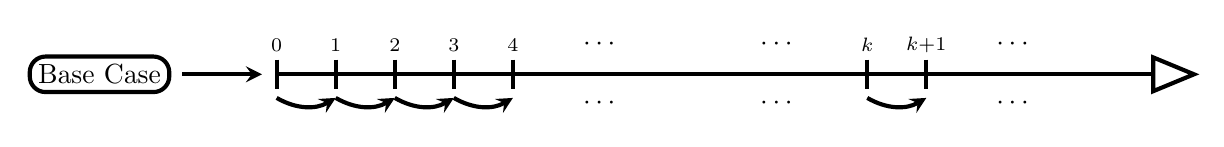
\begin{tikzpicture}[scale=0.75]
            \node[draw,rounded corners=.2cm,inner sep=3pt,line width=1.5pt] (basecase) at (-3, 0) {Base Case};
            \coordinate (0) at (0,0);
            \coordinate (1) at (1,0);
            \coordinate (2) at (2,0);
            \coordinate (3) at (3,0);
            \coordinate (4) at (4,0);
            \coordinate (k) at (10,0);
            \coordinate (k+1) at (11,0);
            \node (n)[isosceles triangle,draw,line width=1.5pt] at (15,0) {};
            
            \draw [line width=1.5pt] (0) -- (n);
            \foreach \lab in {0,1,2,3,4,k,k+1}
                \draw [line width=1.5pt] ($(\lab) + (0,0.25)$) -- ($(\lab) + (0,-0.25)$);
            \foreach \lab in {0,1,2,3,4,k,k+1}
                \node (text\lab) at ($(\lab) + (0,0.5)$) {$\scriptstyle\lab$};

            \node (dotstop1) at ($(4) + (1.5,0.5)$) {$\cdots$};
            \node (dotsbot1) at ($(4) + (1.5,-0.5)$) {$\cdots$};
            
            \node (dotstop2) at ($(k) + (-1.5,0.5)$) {$\cdots$};
            \node (dotsbot2) at ($(k) + (-1.5,-0.5)$) {$\cdots$};

            \node (dotstop3) at ($(k+1) + (1.5,0.5)$) {$\cdots$};
            \node (dotsbot3) at ($(k+1) + (1.5,-0.5)$) {$\cdots$};

            \draw [->,>=stealth,line width=1.5pt] ($(basecase) + (1.4,0)$) to ($(0) + (-0.25,0)$);

            \draw [->,>=stealth,line width=1.5pt,bend right] ($(0) + (0, -0.4)$) to ($(1) + (0, -0.4)$);
            \draw [->,>=stealth,line width=1.5pt,bend right] ($(1) + (0, -0.4)$) to ($(2) + (0, -0.4)$);
            \draw [->,>=stealth,line width=1.5pt,bend right] ($(2) + (0, -0.4)$) to ($(3) + (0, -0.4)$);
            \draw [->,>=stealth,line width=1.5pt,bend right] ($(3) + (0, -0.4)$) to ($(4) + (0, -0.4)$);
            
            \draw [->,>=stealth,line width=1.5pt,bend right] ($(k) + (0, -0.4)$) to ($(k+1) + (0, -0.4)$);
        \end{tikzpicture}
        \label{fig1}
    \end{figure}

More concretely, an inductive proof has three components (adapted from \cite{levet_algorithms_2019}): The base cases, the inductive hypothesis, and the inductive step.

\begin{enumerate}
    \item \textbf{Bases Cases} - We first verify that the statement holds for the minimal case(s) (the ones that start the chain of implications).
    \item \textbf{Inductive Hypothesis} - We want to show that \emph{if} some earlier case(s) satisfy the statement, \emph{then} so do the subsequent cases. The inductive hypothesis is the \emph{if} part of this if-then statement. We do this by assuming that the statement holds for some or all earlier cases.
    \item \textbf{Inductive Step} - We use the inductive hypothesis to prove that the subsequent cases also hold. This is the \emph{then} part of the if-then statement.
\end{enumerate}

As an example, we can then use this proof technique to prove the following proposition.

\begin{proposition}\label{prop1}
    For all \(n \in \ZZ\), we have that:
    \[\sum_{i=0}^n i = \frac{n(n+1)}{2}\]
\end{proposition}
\begin{proof}
    We prove this by induction over \(n \in \ZZ\).
    
    \textbf{Base Case}: We verify that the proposition holds for \(n=0\). We have that \(\sum_{i=0}^0 i = 0\) which is equal to \(\frac{0 \cdot (0 + 1)}{2} = 0\). And thus, the proposition holds for \(n=0\).

    \textbf{Inductive Hypothesis}: Fix some \(k \geq 0\) and suppose that the proposition holds for the \(n=k
    \) case, i.e.,
    \[\sum_{i=0}^k i = \frac{k(k+1)}{2}\]

    \textbf{Inductive Step}: Consider the sum of integers from \(0\) to \(k+1\), we want to show the following.
    \[\sum_{i=0}^{k+1} i = \frac{(k+1)(k+2)}{2}\]
    We do this in the following way using the inductive hypothesis.
    \begin{align*}
        \sum_{i=0}^{k+1} i &= (k+1) + \sum_{i = 0}^{k} i \\
        &= (k+1) + \frac{k(k+1)}{2}\ \ \ \ \text{(by inductive hypothesis)} \\
        &= \frac{2(k+1) + k(k+1)}{2} \\
        &= \frac{k^2 + 3k + 2}{2} \\ 
        &= \frac{(k+1)(k+2)}{2} \\ 
    \end{align*}
    And thus, by induction, the proposition holds for all \(n \in \ZZ\).
\end{proof}

\begin{remark}
    There are many ways to write an inductive hypothesis. For example, we could have said something like ``For some arbitrary \(k \geq 0\), assume that the proposition holds.'' Or we could continue using \(n\) instead of introducing a new variable \(k\). However, be careful. A common mistake is to assume the conclusion. That is, we assume that the entire proposition is true. As an incorrect example, I could have said, ``Suppose that for all \(k \geq 0\), the proposition is true.'' This, however, is incorrect because this is exactly what we are trying to prove (replace \(k\) with \(n\)). This may seem pedantic, but it is important to have the correct wording as otherwise, it can lead to proving incorrect statements. Instead, we want to give a proof for the inductive step for an arbitrary \(k\) by assuming the previous case(s). This distinction is subtle, but important. Using the domino analogy, we only want to suppose that the previous domino(s) fell and not that all the dominos fell.
\end{remark}

The above proof by induction is an example of \emph{weak induction}, the most basic form of induction. In short, weak induction is when we only have a single base case, and the inductive hypothesis only assumes the statement is true for some fixed \(k\).

Now that we have looked at an example, we can formalize this model of induction a bit more. We state the Law (or Axiom) of Weak Induction, which is why induction works.

\begin{definition}[Law of Weak Induction]\label{law_of_weak_ind}
    Let \(P(n)\) be a statement regarding a non-negative integer, \(n \in \ZZ\). If 
    \begin{enumerate}
        \item \(P(0)\) is true and
        \item \(\forall k \geq 0 : P(k) \ra P(k+1)\) is true
    \end{enumerate}
    then \(\forall n \geq 0 : P(n)\) is true.
\end{definition}

This law is not proven and is instead typically given as an axiom. It is for this reason we give it as a definition. Additionally, this is also the reason why you should always say something along the lines of, ``And thus, by induction, the proposition holds for all \(n \in \ZZ\)'' at the end of your inductive proof. 

\begin{remark}
    It is often the case that some statements are not true for small values of \(n < c\) bellow some fixed constant \(c \in \ZZ\) but are true for all \(n \geq c\). We can still use the Law of Weak Induction in these cases. If we seek to prove that \(\forall n \geq c : P(n)\), then we could instead consider the statement \(Q(n) : P(n + c)\). Then proving that \(\forall n \geq 0: Q(n)\) is equivalent to \(\forall n \geq c : P(n)\).
\end{remark}

Finally, we dissect the law of weak induction to understand how our proof of \cref{prop1} fits into this framework. We first prove the base case, this is the \(P(0)\) part. Then we fixed a \(k\) and showed that \(P(k) \ra P(k+1)\). This is both the inductive hypothesis (assuming \(P(k)\) for some fixed \(k\)) and the inductive step (proving the implication itself). Note that we never wrote the \(\forall k \geq 0\) part in the proof. This is because it is implicit. That is, in the inductive hypothesis and inductive step, when we fix an arbitrary \(k\), our proof applies equally as well for any \(k \geq 0\). All in all, this satisfies the second condition, \(\forall k \geq 0 : P(k) \ra P(k+1)\).

To emphasise this point more, let's say we are trying to prove the following proposition. We can then use use the law of induction in a proof in the following way.

\begin{proposition*}[Template Proposition]
    \(\forall n \geq 0 : P(n)\) is true.
\end{proposition*}
\begin{proof}[Template proof]
    We prove that \(\forall n \geq 0 : P(n)\) is true by induction over \(n \geq 0\).
    
    \textbf{Base Case}: Verify \(P(0)\) is true.

    \textbf{Inductive Hypothesis}: Fix a \(k \geq 0\) and suppose that \(P(k)\) is true.

    \textbf{Inductive Step}: Show that \(P(k+1)\) is true assuming the inductive hypothesis (i.e., that \(P(k) \ra P(k+1)\)).

    Then, by the law of (weak) induction, we have proven that \(\forall n \geq 0 : P(n)\).
\end{proof} 
 
\subsection{Strong Induction}

So far, we have looked at weak induction. Another form of induction that is widely used is \emph{strong induction}. In short, strong induction allows us to make a stronger assumption for the inductive hypothesis. That is, we can assume the statement holds for all cases \(m \leq k\), for some fixed \(k\), and not just for \(k\) alone. Before we go further into this technique, we state the Law of Strong Induction.

\begin{definition}[Law of Strong Induction]
    Let \(P(n)\) be a statement regarding a non-negative integer, \(n \in \ZZ\). If
    \begin{enumerate}
        \item \(P(0)\) is true and
        \item \(\forall k \geq 0 : (\forall j \leq k :  P(k)) \ra P(k+1)\) is true
    \end{enumerate}    
    then \(\forall n \geq 0 : P(n)\) is true.
\end{definition}

As we did for weak induction, we can look at a template proof using strong induction.

\begin{proposition*}[Template Proposition]
    \(\forall n \geq 0 : P(n)\) is true.
\end{proposition*}
\begin{proof}[Template proof]
    We prove that \(\forall n \geq 0 : P(n)\) is true by induction over \(n \geq 0\).
    
    \textbf{Base Case}: Verify \(P(0)\) is true.

    \textbf{Inductive Hypothesis}: Fix a \(k \geq 0\) and suppose that \(\forall j \leq k: P(k)\) is true.

    \textbf{Inductive Step}: Show \(P(k+1)\) is true assuming the inductive hypothesis (i.e., \(\left(\forall j \leq k: P(k)\right) \ra P(k+1)\)).

    Then, by the law of (strong) induction, we have proven that \(\forall n \geq 0 : P(n)\).
\end{proof}

Notice the only difference between strong and weak induction is the inductive hypothesis. Pictorially, this makes the chain of implications look like the following.

\begin{figure}[ht]
        \centering
        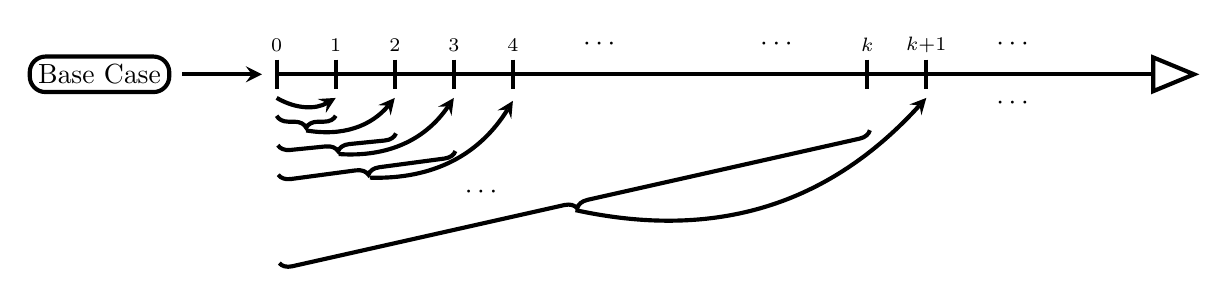
\begin{tikzpicture}[scale=0.75]
            \node[draw,rounded corners=.2cm,inner sep=3pt,line width=1.5pt] (basecase) at (-3, 0) {Base Case};
            \coordinate (0) at (0,0);
            \coordinate (1) at (1,0);
            \coordinate (2) at (2,0);
            \coordinate (3) at (3,0);
            \coordinate (4) at (4,0);
            \coordinate (k) at (10,0);
            \coordinate (k+1) at (11,0);
            \node (n)[isosceles triangle,draw,line width=1.5pt] at (15,0) {};
            
            \draw [line width=1.5pt] (0) -- (n);
            \foreach \lab in {0,1,2,3,4,k,k+1}
                \draw [line width=1.5pt] ($(\lab) + (0,0.25)$) -- ($(\lab) + (0,-0.25)$);
            \foreach \lab in {0,1,2,3,4,k,k+1}
                \node (text\lab) at ($(\lab) + (0,0.5)$) {$\scriptstyle\lab$};

            \node (dotstop1) at ($(4) + (1.5,0.5)$) {$\cdots$};
            
            \node (dotsbot1) at ($0.5*(0) + 0.5*(3) + (2, -2)$) {$\cdots$};
            
            \node (dotstop2) at ($(k) + (-1.5,0.5)$) {$\cdots$};

            \node (dotstop3) at ($(k+1) + (1.5,0.5)$) {$\cdots$};
            \node (dotsbot3) at ($(k+1) + (1.5,-0.5)$) {$\cdots$};

            \draw [->,>=stealth,line width=1.5pt] ($(basecase) + (1.4,0)$) to ($(0) + (-0.25,0)$);
            
            \draw [->,>=stealth,line width=1.5pt,bend right] ($(0) + (0, -0.4)$) to ($(1) + (0, -0.4)$);

            \draw[decorate, decoration={brace, amplitude=1ex, raise=1ex},line width=1.5pt] ($(1) + (0, -0.5)$) -- ($(0) + (0, -0.5)$) node[pos=.5, left=2.5ex] {};
            \draw [->,>=stealth,line width=1.5pt,bend right] ($0.5*(0) + 0.5*(1) + (0, -0.95)$) to ($(2) + (0, -0.4)$);

            \draw[decorate, decoration={brace, amplitude=1ex, raise=1ex},line width=1.5pt] ($(2) + (0, -0.8)$) -- ($(0) + (0, -1)$) node[pos=.5, left=2.5ex] {};
            \draw [->,>=stealth,line width=1.5pt,bend right] ($0.5*(0) + 0.5*(2) + (0.05, -1.35)$) to ($(3) + (0, -0.4)$);

            \draw[decorate, decoration={brace, amplitude=1ex, raise=1ex},line width=1.5pt] ($(3) + (0, -1.1)$) -- ($(0) + (0, -1.5)$) node[pos=.5, left=2.5ex] {};
            \draw [->,>=stealth,line width=1.5pt,bend right] ($0.5*(0) + 0.5*(3) + (0.08, -1.75)$) to ($(4) + (0, -0.45)$);

            \draw[decorate, decoration={brace, amplitude=1ex, raise=1ex},line width=1.5pt] ($(k) + (0, -0.75)$) -- ($(0) + (0, -3)$) node[pos=.5, left=2.5ex] {};
            \draw [->,>=stealth,line width=1.5pt,bend right] ($0.5*(0) + 0.5*(k) + (0.06, -2.3)$) to ($(k+1) + (0, -0.4)$);
        \end{tikzpicture}
        \label{fig2}
    \end{figure}

\begin{remark}
Somewhat surprisingly, strong induction and weak induction are equally as powerful. That is, any proof using strong induction can be converted into a proof using weak induction and vice versa. This is evident by constructing the statement \(Q(n): \forall 0 \leq k \leq n : P(k)\), then using weak induction to prove \(\forall n \geq 0 : Q(n)\) is equivalent to using strong induction to prove \(\forall n \geq 0 : P(n)\). However, in practice, it may be easier to use one over the other. We highlight this in the next example.
\end{remark}

As a side note, in section \cref{sec_loop_inv}, we will see what are called loop invariant proofs, which use weak induction under the hood. That is, they assume only that the loop invariant is true at the start of the loop and then prove that it is true at the end of the loop (or at the start of the next iteration, depending on how you phrase it). In comparison, many proofs for recursive algorithms use strong induction. That is, they assume that the algorithm works for subproblems of smaller sizes.
% See \cref{section_rec_alg_correctness} for more info.

We can then give some examples of using strong induction.

\begin{proposition}
    Let \(F_n\) for \(n \geq 0\) denote the \(n\)th Fibonacci number, which is defined as \(F_0 = 0, F_1 = 1, F_n = F_{n-1} + F_{n-2}\) for \(n \geq 2\). And let \(L_n\) for \(n \geq 0\) denote the \(n\)th Lucas number, which is defined as \(L_0 = 2, L_1 = 1, L_n = L_{n-1} + L_{n-2}\) for \(n \geq 2\). We have that for all \(n \geq 1\),
    \[L_n = F_{n-1} + F_{n+1}\]
\end{proposition}

For reference, we write the first few numbers for both sequences:
\[\begin{array}{c|c|c|c|c|c|c|c|c}
    n   & 0 & 1 & 2 & 3 & 4 & 5 & 6 & 7 \\
    \hline \hline
    F_n & 0 & 1 & 1 & 2 & 3 & 5 & 8 & 13 \\
    \hline
    L_n & 2 & 1 & 3 & 4 & 7 & 11 & 18 & 29 \\
\end{array}\]

\begin{proof}
    We prove this by strong induction over \(n \geq 1\).
    
    \textbf{Base Case}: We verify that the proposition holds for \(n=1\) and \(n=2\). First, we can verify that \(L_1 = 1\) and \(F_0 + F_2 = 0 + 1 = 1\). Next, we can verify that \(L_2 = 3\) and \(F_1 + F_3 = 1 + 2 = 3\). And thus, the proposition holds for \(n=1\) and \(n=2\).

    \textbf{Inductive Hypothesis}: Fix some \(k \geq 2\) and suppose that the proposition holds for the \(k\) and \(k-1\) cases:
    \[L_k = F_{k-1} + F_{k+1}\]
    \[L_{k-1} = F_{k-2} + F_{k}\]

    \textbf{Inductive Step}: Consider the \((k+1)\)th Lucas number, which we want to show is \(L_{k+1} = F_{k} + F_{k+2}\). We do this in the following way.
    \begin{align*}
        L_{k+1} &= L_{k} + L_{k-1} & \text{(by definition of the Lucas numbers)} \\
        &= F_{k-1} + F_{k+1} + F_{k-2} + F_{k} & \text{(by inductive hypothesis)} \\
        &= F_{k} + F_{k+2} & \text{(by definition of the Fibonacci numbers)}
    \end{align*}
    % \[\begin{array}{rll}
    %     L_{k+1} \!\!\!\! &= L_{k} + L_{k-1} & \text{(by definition of the Lucas numbers)} \\
    %     &= F_{k-1} + F_{k+1} + F_{k-2} + F_{k} & \text{(by inductive hypothesis)} \\
    %     &= F_{k} + F_{k+2} & \text{(by definition of the Fibonacci numbers)}
    % \end{array}\]
    And thus, by induction, the proposition holds for all \(n \geq 1\).
\end{proof}

\begin{remark}
    In this proof, we used two base cases and supposed the proposition held for both \(n=k\) and \(n=k-1\) for some fixed \(k \geq 2\), but why is this needed? You will notice that in the inductive step, we applied the inductive hypothesis to both \(L_k\) and \(L_{k-1}\). If we only supposed that the proposition held for \(n=k\), then we would be left with \(L_{k+1} = F_{k-1} + F_{k+1} + L_{k-1}\), which wouldn't help us prove the proposition for \(n=k+1\). Next, for the base cases, if we were only to have one base case, for \(n=1\), then the inductive hypothesis would have to consider some fixed \(k \geq 1\). For the smallest value of \(k=1\), this would have us suppose that \(L_0 = F_{-1} + F_{1}\), which doesn't make sense as negative Fibonacci numbers haven't been defined in this proposition. We note that this still fits into the framework given by the law of strong induction as \(P(1)\) implies that \(P(0) \ra P(1)\). %As a general rule of thumb, the number of required base cases equals the number of assumptions you make in the inductive hypothesis (this isn't always true, but it often a good rule of thumb to start with).
\end{remark}

\subsection{A Longer Example}

Next, we will look at the tournament ranking problem 
\footnote{Quick integrity check. This problem is often given as homework; if you use this solution at any step while doing your homework for a future or current class, you should always cite your sources.}.
So far, all the proofs in this document have only concerned numerical equalities. However, this is a computer science class, and so we want to prove things that are more relevant to algorithms. The tournament ranking is a nice introduction to this.

\begin{proposition}[The Tournament Ranking Problem]
    Consider a tennis tournament of \(n \geq 1\) players, denoted by \(\left\{P_1, P_2, \dotsc, P_n\right\}\). For each pair of distinct players, say \((P_i, P_j)\) (for \(i \neq j\)), they play a match where one player wins (there are no ties). We say \(P_i \prec P_j\) if player \(P_j\) beats \(P_i\) in their match. Then for any outcome of the \(\binom{n}{2}\) matches, there is always an ordering of the players:
    \[P_{i_1} \prec P_{i_2} \prec \cdots \prec P_{i_n}\]
    Here, \((i_1, i_2, \dotsc, i_n)\) denotes a permutation of \((1, 2, \dotsc, n)\). Note, we do \emph{not} require that an ordering be transitive, that is, for an ordering \(P_1 \prec P_2 \prec P_3\) does, this does \emph{not} imply \(P_1 \prec P_3\), rather only that \(P_1 \prec P_2\) and \(P_2 \prec P_3\).
\end{proposition}

\vspace{0.1in}

Before we prove this, it is useful to give the idea of the proof. That is, for our tournament of \(n\) players, which, for notation we will call \(\text{PLAYERS} = \left\{P_1, P_2, \dotsc, P_n\right\}\), we fix player \(P_1\) and consider all the players that lost to player \(P_1\) and all the players that beat \(P_1\). That is, we consider all the players that can go where the \(??\)s are:
\[?? \prec P_1 \prec ??\]
Furthermore, the number of players that can go where the \(??\)s are is strictly less than \(n\) as they can't include \(P_1\). This defines a recursive structure of the problem. Namely, if we can find an ordering of these subsets of players and put them where the question marks are, we would get an ordering for all \(n\) players.

To make the proof easier, we will consider the base case to be when there are no players in the tournament. Even though we only need to prove this proposition for \(n \geq 1\), we will find it to be much easier to prove it for \(n \geq 0\). This may seem weird at first, but everything works out as far as the induction step is concerned.

\begin{proof}
    We prove this by strong induction over the number of players in the tournament, \(n \geq 0\).
    
    \textbf{Base Case}: We verify that there exists an ordering for no player, \(\emptyset\). The ordering is nothing.

    \textbf{Inductive Hypothesis}: Fix some \(k \geq 0\) and suppose that for any tournament of \(0 \leq m \leq k\) players there exists an ordering of the players.

    \textbf{Inductive Step}: Consider a tournament of \(k+1\) players and let \(\text{PLAYERS} = \left\{P_1, P_2, \dotsc, P_k, P_{k+1}\right\}\) be the set of the players. We then fix \(P_1\) and consider the set of players that lost to \(P_1\), which we will call \(L\), and the set of players that beat \(P_1\), which we will call \(W\). These sets can be defined by 
    \[L = \{P \in \text{PLAYERS}\ |\ P \prec P_1\}\]
    \[W = \{P \in \text{PLAYERS}\ |\ P_1 \prec P\}\]

    Because \(P_1 \notin L\) and \(P_1 \notin W\) we have that \(s = |L| \leq k\) and \(t = |W| \leq k\). Furthermore, because no player can both lose and win to \(P_1\) and every player had a match with \(P_1\), they are disjoint, and their union is all players minus \(P_1\). We can then use the induction hypothesis to get an ordering of the players in \(L\) and \(W\) (that is, we consider ``sub-tournaments'' of only the matches between the players in \(L\) and \(W\)). Let the orderings for \(L\) and \(W\), guaranteed by the inductive hypothesis, be given by the following, respectively:
    \[P_{\ell_1} \prec P_{\ell_2} \prec \cdots \prec P_{\ell_s}\]
    \[P_{w_1} \prec P_{w_2} \prec \cdots \prec P_{w_s}\]
    Finally, we can construct the final ordering as follows. Note, if either \(L\) or \(W\) are the empty set, then we ignore their orderings and let \(P_1\) be at one or both of the ends of the ordering.
    \[P_{\ell_1} \prec \cdots \prec P_{\ell_s} \prec P_1 \prec P_{w_1} \prec \cdots \prec P_{w_s}\]
    All that is left to check is that \(P_{\ell_s} \prec P_1\) and \(P_1 \prec P_{w_1}\). These follow from the fact that \(P_{\ell_s} \in L\) and thus lost to \(P_1\) and that \(P_{w_1} \in W\) and thus beat \(P_1\).

    Thus, by induction, there is always an ordering for any tournament of \(n \geq 1\) players.
\end{proof}

\begin{remark}
    In many ways, the inductive step can be seen as proving the correctness of a recursive algorithm for finding an ordering. This algorithm is a divide-and-conquer style strategy that can be roughly written in the following way: We first divide the problem into the losing and winning sets, then we find an ordering for them recursively, and finally, we combine them together to get an ordering for the whole set. Then, proving the proposition is equivalent to proving the correctness of this algorithm (which is written in pseudo-code below). Note we store this ordering in a list data structure that supports list concatenation with the \(+\) operator.
    \begin{algorithm}[Tournament Ranking Algorithm] \phantom{}\label{alg_tourn_ranking}
    
    \begin{center}
    \begin{minipage}{.5\linewidth}
    \begin{algorithmic}[1]
        \Procedure{\textsc{TournamentRanking}}{\text{PLAYERS}}
            \If{\(\text{PLAYERS} = \emptyset\)} 
                \Return \([\;]\)
            \Else
                \State fix \(P_1 \in \text{PLAYERS}\)
                \State \(L \leftarrow \{P \in \text{PLAYERS}\ |\ P \prec P_1\}\)
                \State \(W \leftarrow \{P \in \text{PLAYERS}\ |\ P_1 \prec P\}\)

                \State \(L_{\text{ord}} \leftarrow \textsc{TournamentRanking}(L)\)
                \State \(W_{\text{ord}} \leftarrow \textsc{TournamentRanking}(W)\)
                
                \State \textbf{return} \(L_{\text{ord}} + [P_1] + W_{\text{ord}}\)
            \EndIf 
        \EndProcedure
    \end{algorithmic}
    \end{minipage}
    \end{center}
    \end{algorithm}
\end{remark}

\subsection{Problems/Exercises}

This is a list of some of my go to problems. I have the solutions for some of them.

\begin{problem}
    Prove the following for all \(n \in \ZZZ\):
    \[\sum_{i=1}^n i (i+1) = \frac{n(n+1)(n+2)}{3}\]
\end{problem}

\begin{problem}
    Prove the following:
    Let \(n \in \ZZZ\), then for two sequences of positive numbers, \((a_i)_{i \in [n]}\) and \((b_i)_{i \in [n]}\) we have that
    \[\min_{i \in [n]} \left(\frac{a_i}{b_i}\right) \leq \frac{\sum_{i = 1}^n a_i}{\sum_{i = 1}^n b_i} \leq \max_{i \in [n]} \left(\frac{a_i}{b_i}\right)\]

    [Hint: First prove the \(n=2\) case, then break up your inductive case into two cases that allow you to use the result of the \(n=2\) case directly. Note, your base case should still be for \(n=1\).]
\end{problem}

\begin{problem}
    Prove the following: Let \(F_n\) for \(n \geq 0\) denote the \(n\)th Fibonacci number. Fix an \(n \in \ZZ\), then we have the following
    \[\sum_{i = 0}^n F_n = F_{n+2} - 1\]
\end{problem}

\begin{problem}
    Prove that all connected graphs on \(n\) vertices have at least \(n-1\) edges.
\end{problem}

\begin{problem}
    Prove that any planar graph can be colored in 6 colors. You may use, without proof, the fact that every planar graph always has at least one vertex with degree no more than 5 (this is evident by bounding the average degree using Euler's formula, \(|V| - |E| + |F| = 2\), and the fact that \(2 |E| \geq 3 |F|\), which in turn follows from the hand shake lemma).
    % Strengthen your proof to show that every planar graph can be colored in 5 colors. This will require a proof by contradiction in you're inductive step. Assume that the graph can't be colored in 5 colors but the subgraph in the inductive hypothesis can be colored in 5 colors. Show that this leads to a contradiction with the fact that the graph is planar. 
\end{problem}

\begin{problem}[I'll take \(n\) please]
    You're favorite dumpling shop only sells dumplings in amounts of 3,5, or 8. However, you are very hungry and would like an arbitrary number of dumplings. You recall that your friend once said they used a trick to order exactly \(9\) or \(10\) dumplings by ordering three orders of three or two orders of five. Prove that for any value of \(n \geq 8\) there is a way to order exactly that many dumplings.
\end{problem}

\section{Loop Invariant Proofs}\label{sec_loop_inv}

One common variant of induction seen in computer science is a loop invariant proof. In short, these are used when an algorithm has a loop, and you want to prove something about the algorithm. For the proof, you do (weak) induction over the loop to prove that some statement that depends on the loop number is true for each loop and after the loop has terminated. This statement is referred to as a loop invariant.

In addition to a loop invariant, we will also have a statement that determines whether we are still in the loop or not. We will call this the loop condition. If our algorithm is a loop of the form \textbf{while} \(C(i)\) \textbf{do}, then \(C(i)\) is the loop condition. Here, \(i\) is the loop number.

One common confusion with loop invariants is whether the loop invariant should be true at the beginning of the loop or at the end. It turns out that either type of loop invariant works, and, in fact, they are equivalent up to a `\(+1\)' in the loop number. However, there are subtle differences between how the proof is set up using two models. In this section, we discuss both. We suggest that you pick one model and stick with it in your own proofs. It is rarely the case that one is easier than the other, as was true for weak and strong induction. To paint a picture of what a loop invariant is, consider the following bare-bones example.

\begin{example}\label{ex_loop_inv_b_e}
    We break down an iterative algorithm into parts that will help us understand the structure of a loop invariant. We use ``Initialization Step,'' ``Loop Step,'' and ``Termination Step'' to denote arbitrary code that you would have to reason about in the proof.
    
    Any loop can be converted to have the structure of the following example. We let {\color{red}\(I_b(i)\)} denote the loop invariant that is true at the beginning of the loop and {\color{blue}\(I_e(i)\)} be the loop invariant that is true at the end of the loop. Additionally, \(i\) will denote the iteration number, which is explicit in the following example but may not be in general.
    \begin{center}
    \begin{minipage}{.5\linewidth}
    \begin{algorithmic}[1]
        \State Initialization Step
        \State {\color{blue}\textbf{assert} \(I_e(0)\)}
        \State \(i \leftarrow 1\)
        \While{$C(i)$}
            \State {\color{red}\textbf{assert} \(I_b(i)\)}
            \State Loop Step
            \State {\color{blue}\textbf{assert} \(I_e(i)\)}
            \State \(i \leftarrow i + 1\)
        \EndWhile
        \State {\color{red}\textbf{assert} \(I_b(i)\)}
        \State Termination Step
    \end{algorithmic}
    \end{minipage}
    \end{center}
Note that while both variations serve that same purpose, we don't, in general, have that \({\color{red}I_b(i)} = {\color{blue}I_e(i)}\) but instead have that \({\color{red}I_b(i+1)} = {\color{blue}I_e(i)}\). Moreover, \(\color{red}I_b(0)\) need not be defined and same for \(\color{blue}I_e(n+1)\), where \(n\) is the last time that \(C(n)\) is true, i.e., \(C(n+1)\) is false. 
\end{example}

Before formally defining a loop invariant, we will want a little more structure on the statement, \(C(i)\). Even though it is never used in the loop, it will be useful to have \(C(0)\) defined to be true. Moreover, when the loop terminates, i.e., \(C(n)\) is false for some \(n \geq 1\), we will want to enforce that all larger integers, \(k \geq n\), \(C(k)\) also be false. That is, we will enforce that \(\forall n \geq 1 : \lnot C(n) \ra \forall k \geq n : \lnot C(k)\). We note that neither of these has any bearing on how \(C(i)\) is used in the loop itself, but nonetheless, we do this to make the mathematical definitions easier.

With the loop condition, \(C(i)\), in hand, we can now formally define a loop invariant. We take special consideration as to whether it should be true at the start or the end of the loop, even though both are equivalent, up to how they relate to \(C(i)\).

\begin{definition}[Loop Invariant]
    A \emph{loop invariant} is a statement \(I(n)\) regarding a non-negative integer \(n \in \ZZ\) that is true until \(C(n)\) is false. More formally, if \(I(n)\) is defined to be true at the beginning of the loop, then \(I(n)\) is a loop invariant if \(\forall n \geq 1 : C(n-1) \ra I(n)\). If, on the other hand, \(I(n)\) is defined to be true at the end of the loop, then \(I(n)\) is a loop invariant if \(I(0) \land \forall n \geq 1 : C(n) \ra I(n)\).
\end{definition}

\begin{remark}
    In both cases, you should think of \(C(n)\) as determining if the loop will be run. In the first case (beginning of loop case), we want the loop invariant to be true during the loop and after the loop has terminated. So if \(n\) is the first value that makes \(C(n)\) false, then we still want \(I(n)\) to be true. In the other case (end of loop case), if \(C(n)\) is false, then we wouldn't have run that loop, and thus we only ensure that \(I(n-1)\) is true. 
\end{remark}

In order to prove a loop invariant, we use induction. However, this time, we have to incorporate the loop condition into the proof. For this, we consider the modified law of (weak) induction. We note that it is, again, equally as powerful as the law of (weak) induction. However, we state the following as propositions to emphasize how they follow from the Law of induction, \cref{law_of_weak_ind}. We, of course, continue to break this down into two cases, whether the loop invariant is defined to be true at the beginning or the end of the loop.

\begin{proposition}[Beginning of Loop Case]\label{law_loop_inv_b}
    Let \(I(n)\) and \(C(n)\) be statements regarding a non-negative integer, \(n \in \ZZ\), where \(C(0)\) is defined to be true and \(\forall n \geq 0: \lnot C(n) \ra \forall k \geq n : \lnot C(k)\). Then, if
    \begin{enumerate}
        \item \(I(1)\) is true and
        \item \(\forall k \geq 1 : C(k) \land I(k) \ra I(k+1)\) is true
    \end{enumerate}    
    then \(\forall n \geq 1 : C(n-1) \ra I(n)\) is true (i.e., \(I(n)\) is loop invariant, at the beginning of the loop).
\end{proposition}

Next, we give the variant of \cref{law_loop_inv_b} for loop invariants that are true at the end of the loop.

\begin{proposition}[End of Loop Case]\label{law_loop_inv_e}
    Let \(I(n)\) and \(C(n)\) be statements regarding a non-negative integer, \(n \in \ZZ\), where \(C(0)\) is defined to be true and \(\forall n \geq 0: \lnot C(n) \ra \forall k \geq n : \lnot C(k)\). Then, if
    \begin{enumerate}
        \item \(I(0)\) is true and
        \item \(\forall k \geq 0 : C(k+1) \land I(k) \ra I(k+1)\) is true
    \end{enumerate}    
    then \(\forall n \geq 0 : C(n) \ra I(n)\) is true (i.e., \(I(n)\) is loop invariant, at the end of the loop).
\end{proposition}

\begin{remark}
    We quickly remark on the differences in the inductive steps for the two definitions. In \cref{law_loop_inv_b}, the inductive hypothesis is \(I(k) \land C(k)\). You can think of this as saying that if the loop invariant is true at the beginning of loop \(k\) and the loop will be executed for iteration \(k\) (i.e., \(C(k)\)), then the loop invariant should be true at the start of the next iteration or after termination.

    Similarly, in \cref{law_loop_inv_e} the inductive hypothesis is \(I(k) \land C(k+1)\). You can think of this as saying that if the loop invariant is true at the end of the \(k\)th loop and the loop will be executed for one more iteration (i.e., \(C(k+1)\)), then the loop invariant should be true at the end of the next iteration.
\end{remark}

As with before, we give a template proof using this structure. For now, we only give it for \cref{law_loop_inv_b}. The other variant is used in the proof of \cref{prop_correct_lsearch}.

\begin{proposition*}[Template Proposition]
    \(\forall n \geq 1 : C(n-1) \ra I(n)\) is true (i.e., \(I(n)\) is a loop invariant that is true at the beginning of the loop and after termination).
\end{proposition*}
\begin{proof}[Template proof]
    We prove that \(\forall n \geq 1 : C(n-1) \ra I(n)\) is true by induction over \(n \geq 1\).
    
    \textbf{Base Case}: Verify \(I(1)\) is true.

    \textbf{Inductive Hypothesis}: Fix a \(k \geq 1\) and suppose that \(C(k) \land I(k)\) is true.

    \textbf{Inductive Step}: Show that \(C(k) \land I(k) \ra I(k+1)\).

    Then, by the law of (weak) induction, we have proven that \(\forall n \geq 1 : C(n-1) \ra I(n)\).
\end{proof}
\zacktodo{Interestingly, if we also prove that \(C(n)\) will be false for some finite constant \(n_0\), then we never actually have to use the law of induction. However, it is often the case that \(C(n)\) will depend on other variables and thus it could be the case that no constant exists.}

Now that we have discussed proving that a loop invariant is a loop invariant, we will want to use it to prove the correctness of an algorithm. This follows in three parts. First, you need to identify a loop invariant. Second, prove the loop invariant. Finally, use the loop invariant and, in particular, the one after the algorithm terminates, to prove the correctness of the algorithm. In order to do this last step, you will also need to prove that the algorithm terminates, i.e., that \(\exists n \geq 0 : \lnot C(n)\).

\begin{remark}
    Often a loop invariant proof is phrased in three parts. Initialization, Maintenance, and Termination. The first two steps are equivalent to proving that a loop invariant is indeed a loop invariant. That is, they are the base case and the inductive step, respectively. Then the termination step has you prove that the algorithm terminates and then use the loop invariant to prove the correctness of the algorithm. While this structure is common, we won't use it explicitly in these notes.
\end{remark}

To make this more clear and to finish this section, we give an example proof of correctness using loop invariants. For this, we consider the following simple algorithm.

\begin{algorithm}[Linear Search Algorithm] \phantom{}\label{alg_lsearch}
\begin{center}
\begin{minipage}{.5\linewidth}
\begin{algorithmic}[1]
    \Procedure{\textsc{LinearSearch}}{$A[1,\dotsc, n],x$}
        \For{$k$ from $1$ to $n$}
            \If{$A[k] = x$}
                \State \textbf{return} \(k\)
            \EndIf
        \EndFor
        \State \textbf{return} \(-1\)
    \EndProcedure
\end{algorithmic}
\end{minipage}
\end{center}
\end{algorithm}

We will prove the following.

\begin{proposition}\label{prop_correct_lsearch}
    The linear search algorithm, given in \cref{alg_lsearch}, correctly returns an index \(k \in [n] = \{1,\dotsc,n\}\) such that \(A[k] = x\) or \(-1\) is no such index exists. 
\end{proposition}

\begin{proof}
    We do this using the following loop invariant that is true before the loop and at the end of each loop, \(I(k) : \forall i \in [k] = \{1, \dotsc, k\} : A[i] \neq x\). In words, the subarray \(A[1,\dotsc,k]\) does not contain the element \(x\) anywhere. We also define the loop condition to be, \(C(k) : k \leq n \land A[k] \neq x\). We then prove this is a valid loop invariant by induction over \(k \geq 1\). That is, we prove that \(\forall k \geq 1 : C(k) \ra I(k)\).
    
    \textbf{Base Case}: We first verify that \(I(0) : \forall i \in [0] = \emptyset : A[i] \neq x\) is true. This is the case because the universal quantifier is vacuously true.

    \textbf{Inductive Hypothesis}: Fix a \(k \geq 0\) and suppose that \(C(k+1) \land I(k)\) is true. That is \(k+1 \leq n \land A[k+1] \neq x \land \forall i \in [k] = \{1, \dotsc, k\} : A[i] \neq x\).

    \textbf{Inductive Step}: We then show that the inductive hypothesis implies that \(I(k+1) = \forall i \in [k+1] = \{1, \dotsc, k+1\} : A[i] \neq x\) is true. This follows directly from the loop invariant and the loop condition.
    \begin{align*}
        k+1 \leq n \land A[k+1] \neq x \land \forall i \in [k] : A[i] \neq x &\rightarrow \forall i \in [k] : A[i] \neq x \land A[k+1] \neq x \\
        &\rightarrow \forall i \in [k+1] : A[i] \neq x
    \end{align*}

    Then, by induction, we have proven that \(\forall k \geq 1 : C(k) \ra I(k)\), i.e., that \(I(k)\) is a loop invariant, which is true at the end of the loop. 

    Finally, we prove the claim. In particular, the loop must terminate as we add one to \(k\) after each iteration, and so eventually, \(k > n\) or \(A[k] = x\). If \(k > n\), then the loop invariant for \(I(n)\) tells us that \(x \notin A\), and thus the algorithm will correctly return \(-1\). If \(A[k] = x\), then the algorithm will terminate and return \(k\), as it found such an index.
\end{proof}

\begin{remark}
    Interestingly, the loop invariant was primarily used to prove the correctness of the case where the algorithm returns \(-1\). This is to say that the loop invariant had little to do with the exact statement of the proposition we were proving and instead implied the proposition with some extra work. Additionally, note that, while \(A[k] \neq x\) wasn't in the loop directly, it is important for determining when the loop terminates. Therefore, we need to add it it the loop condition. 
\end{remark}

\subsection{Problems/Exercises}

\begin{problem}
    Prove that the alternate linear search algorithm, given bellow, correctly returns an index \(k \in [n] = \{1,\dotsc,n\}\) such that \(A[k] = x\) or \(-1\) is no such index exists. 

    \begin{algorithm*}[Alternate Linear Search Algorithm] \phantom{}%\label{alg_lsearch_2}
        \begin{center}
        \begin{minipage}{.5\linewidth}
        \begin{algorithmic}[1]
            \Procedure{\textsc{LinearSearch}}{$A[1,\dotsc, n],x$}
                \State \(i \leftarrow -1\)
                \For{$k$ from $1$ to $n$}
                    \If{$A[k] = x$}
                        \State \(i \leftarrow k\)
                    \EndIf
                \EndFor
                \State \textbf{return} \(i\)
            \EndProcedure
        \end{algorithmic}
        \end{minipage}
        \end{center}
        \end{algorithm*}
\end{problem}

\begin{problem}\label{prob_bin_search_li}
    Prove that the iterative version of binary search works correctly. That is, for any sorted (ascending) input array \(A[1,\dotsc, n]\) on \(n\) elements of \(\Z\) and an element \(x \in \Z\), the binary search algorithm given bellow will find an index \(i \in [n] = \{1, \dotsc, n\}\) such that \(A[i] = x\) or if none exist then the algorithm gives \(-1\).

    \begin{algorithm*}[Binary Search Algorithm] \phantom{}%\label{alg_bsearch}
        \begin{center}
        \begin{minipage}{.5\linewidth}
        \begin{algorithmic}[1]
            \Procedure{\textsc{BinarySearch}}{$A[1,\dotsc, n], x$}
                \State \(\ell \leftarrow 1\)
                \State \(r \leftarrow n\)
    
                \While{$\ell \leq r$}
                    \State \(m \leftarrow \ell + \left\lfloor\frac{r - \ell}{2}\right\rfloor\)
        
                    \If{$A[m] = x$}
                        \State \textbf{return} \(m\)
                    \ElsIf{$A[m] < x$}
                        \State \(\ell \leftarrow m + 1\)
                    \Else
                        \State \(r \leftarrow m - 1\)
                    \EndIf
                        
                \EndWhile	
                   
                \State \textbf{return} \(-1\)
            \EndProcedure
        \end{algorithmic}
        \end{minipage}
        \end{center}
        \end{algorithm*}
\end{problem}

\begin{problem}
    You are given a stack of origami paper, all of different sizes. You want to sort them by their size so that you have the largest paper on the bottom and the smallest on top. You can pick up only the top few papers, flip them, and then put them back on top of the pile. You have the idea to
    \begin{enumerate}
        \item Find the largest piece of paper, then flip it and the papers above it.
        \item Flip the pile starting at the \(i\)th paper from the bottom; here \(i\) is the number of times you did this step.
        \item Repeat steps (1) and (2) until the stack is sorted, but for (1), find the next largest paper.
    \end{enumerate}
    Prove this algorithm terminates and that it correctly sorts the papers.
\end{problem}

% \section{Proving the Correctness of Recursive Algorithms (Unfinished)}\label{section_rec_alg_correctness}

% In this section we look more closely at applying the proof by induction technique to recursive algorithms. As we saw with \cref{alg_tourn_ranking}, a strong induction proof often can been seen as proving the correctness of a recursive algorithm. This is primarily because our proof gave a construction of a ranking. In particular, each step in the proof mirrored a step in an algorithm. Moreover, when we used the inductive hypothesis, we assumed that such a construction exist on a smaller tournament sizes. In algorithm terms, we assumed that our algorithm would work for smaller input sizes.

% We can then dissect the parts in a recursive algorithm. Many recursive algorithm can be categorized as a divide-and-conquer algorithm. These have three parts.
% \begin{enumerate}
%     \item \textbf{Divide:} Divide the input into sub-problems of strictly smaller size.
%     \item \textbf{Conquer:} Recursively call the algorithm on these sub-problems.
%     \item \textbf{Combine:} Combine the results of the sub-problems to get a solution for the whole problem.
% \end{enumerate}
% When the problem can't be divided into smaller problems we would have a base case that does simple calculations, usually on instances with constant size. 

% We can then see how this framework mirrors the proof by induction paradigm, and in particular that of strong induction. That is, the correctness of the algorithm depends on the correctness of the base case and the correctness an of the algorithm on arbitrary sized input if it is correct for smaller inputs.

% Consider the following sorting algorithm. We will prove the correctness using proof by induction. Here, by correct, we mean that it correctly sorts a list of numbers.

\defbibnote{note}{For a more in-depth resource, Richard Hammacks's \emph{Book of Proof} (Chapter 10) is great \cite{hammack_book_2019}. Additionally, one of my past TAs, Michael Levet, has an excellent resource on mathematics in computer science \cite{levet_algorithms_2019}, the first chapter of which is on proof by induction.

Inspiration for earlier drafts of these notes came, in part, from these two sources.}

\printbibliography[title={Additional Reading and Reference},prenote=note,heading=bibintoc]

\end{document}
